%% This is file `DEMO-TUDaThesis.tex' version 4.03 (2025-04-02),
%% it is part of
%% TUDa-CI -- Corporate Design for TU Darmstadt
%% ----------------------------------------------------------------------------
%%
%% Copyright (C) 2018--2025 by Marei Peischl <marei@peitex.de>
%%
%% ============================================================================
%% This work may be distributed and/or modified under the
%% conditions of the LaTeX Project Public License, either version 1.3c
%% of this license or (at your option) any later version.
%% The latest version of this license is in
%% http://www.latex-project.org/lppl.txt
%% and version 1.3c or later is part of all distributions of LaTeX
%% version 2008/05/04 or later.
%%
%% This work has the LPPL maintenance status `maintained'.
%%
%% The current maintainer of this work is
%%   Marei Peischl <tuda-ci@peitex.de>
%%
%% The development repository can be found at
%% https://github.com/tudace/tuda_latex_templates
%% Please use the issue tracker for feedback!
%%
%% If you need a compiled version of this document, have a look at
%% http://mirror.ctan.org/macros/latex/contrib/tuda-ci/doc
%% or at the documentation directory of this package (if installed)
%% <path to your LaTeX distribution>/doc/latex/tuda-ci
%% ============================================================================
%%
% !TeX program = lualatex
%%

% Enable PDF/A via pdfmanagement and no longer via pdfx
\DocumentMetadata{
	pdfstandard=a-2b,
	pdfversion=1.7,% 2.0 is possible as well, but PDF/A-2b requires < 2.0
	lang=en,
}

\documentclass[
	german,% Main language as global option
	accentcolor=9c,% Choose accent color: For a list of available colors see the full tudapub documentation
	ruledheaders=section,% Section levels above this one will follow the ruled layout
	class=report,% Choose the base document class. Will choose the matching KOMA-Script class
	thesis={type=bachelor},% Thesis. For PhD thesis have a look at DEMO-TUDaPhd example file
	fontsize=11pt,% Basic font size. CI default setting of 9pt is too small for theses
	parskip=half-,% Use a parskip instead of indent, see KOMA-Script documentation
	custommargins=false,% Calculate margins using typearea
	marginpar=false,% Disable marginpar
	BCOR=5mm,% Binding correction
% 	accept-missing-logos=true,% No error in case logo files are not available
 	logofile=tools/logo-installation/TUDa-logos/tuda_logo.png,% In case logo should be replaced
]{tudapub}


%%%%%%%%%%%%%%%%%%%
% Language setup
%%%%%%%%%%%%%%%%%%%
\usepackage[english]{babel}
\usepackage{microtype}
\usepackage[autostyle]{csquotes}% \enquote, to simplify use of quotation marks

%%%%%%%%%%%%%%%%%%%
% Bibliography
%%%%%%%%%%%%%%%%%%%
\usepackage[sorting=none, citestyle=numeric-comp]{biblatex}
\addbibresource{ref.bib}% File name of BibTeX database

%%%%%%%%%%%%%%%%%%%
% Package suggestions for tables
%%%%%%%%%%%%%%%%%%%
\usepackage{array}% Fundamental tools for tables. Is automatically loaded by the following packages
%\usepackage{tabularx}% Tables with flexible columns to achieve fixed width
%\usepackage{longtable}% Tables across multiple pages
%\usepackage{xltabular}% Tables with fixed width spanning multiple pages
%\usepackage{booktabs}% Improved layout for horizontal rules in tables

%%%%%%%%%%%%%%%%%%%
% Package suggestions math
%%%%%%%%%%%%%%%%%%%
\usepackage{mathtools}% Extended version of amsmath
\usepackage{amssymb}% Additional symbols
\usepackage{siunitx}% Numbers and Units

\usepackage{subcaption}
\usepackage{tikz}
\usepackage{pgfplots}
\pgfplotsset{compat=1.18} % You can adjust the version as needed


\hypersetup{% Metadata adjustments, in case these are not set, the data provided for \maketitle will be used
	pdfauthor=Marei Peischl (peiTeX),
	pdfcreationdate=2024-05-03,
	pdfkeywords={TU Darmstadt; Corporate Design; LaTeX}
}

\title{Removal of undesired resonances of Terahertz antennas by inclusion of resistive feeds}
\author{Jakob Schmidt}
\reviewer{Prof. Dr. rer. nat. Sascha Preu \and Florian Bek M.Sc.}

% The following elements will be placed on the title page
\department{etit}% If defined the shorthand will be replaced by the full name otherwhise it's used directly.
\institute{Institute for Microwave Engineering and Photonics}
\group{Terahertz Devices and Systems}

\submissiondate{\today}
\examdate{\today}

%\tuprints{printid=XXXX,year=2022,license=cc-by-4.0}% License information for TUprints

\begin{document}

\maketitle

%% The affidavit was deactivated by default at the request of Department II.
%% According to the department, the legally binding text can be found at https://www.tu-darmstadt.de/studieren/studierende_tu/studienorganisation_und_tucan/hilfe_und_faq/artikel_details_de_en_37824.de.jsp
%%  The docx file should be used, printed out, signed, scanned and then integrated.
%% The easiest way to do this is to use the pdfpages package.
%%
%% For compatibility reasons for the other templates, the function is still available.
%% \affidavit[signature-image={\includegraphics[width=\width,height=1cm]{example-image}}, <there may be additional options here>]

\tableofcontents
% Additional lists like \listoffigures or acronyms might be added here
\listoffigures
\newpage

\chapter{Introduction}
Inbetween the microwave and infrared (IR) frequencies of the electromagnetic (EM) spectrum lies Terahertz (THz) radiation (make ref to figure) \cite{zhangIntroductionTHzWave2010}. THz radiation refers to the frequency (wavelength) spectrum ranging from \num{100} \si{\giga\hertz} (\num{3} \si{\milli\meter}) up to \num{10} \si{\tera\hertz} (\num{30} \si{\micro\meter}) \cite{PrinciplesTerahertzScience2009}. While microwave and infrared sources are able to provide high magnitudes of power at those frequencies, there has been a lack of efficient and feasible high power sources in the THz range \cite{perkowitzNavigatingTerahertzGap2020}. This has led to the common reference to the THz range as the \enquote{THz gap} (e.g. see \cite{dhillon2017TerahertzScience2017}, \cite{williamsFillingTHzGap2006}, \cite{zhangAdvancesTerahertzTechnology2021}). THz radiation shows potential in many fields. Thus tremendous efforts have been made in the last two decades to narrow the \enquote{THz gap} \cite{preuTunableContinuouswaveTerahertz2011}. Narrowing the gap has been achieved from both the microwave and the optical side. Advances have been made by extending the high frequency cut-off in purely electronic RF devices, decreasing the lower cut-off frequencies of purely optical IR devices or even by combining the two approaches. \textbf{TODO: citations}.

\textbf{TODO Überleitung zu TDS}


In many fields such as pharmaceutics \cite{huangProgressApplicationTerahertz2023}, materials sciences \cite{zhangApplicationTHzTDSCharacterization2024}, chemistry \cite{fischerChemicalRecognitionTerahertz2005} and many more (e.g. see \cite{petrovMobileNearfieldTerahertz2023, markelzPerspectiveTerahertzApplications2022,TerahertzSpectroscopyIts2011,kleine-ostmannReviewTerahertzCommunications2011}), THz-TDS has proven to be a valuable technique. 

\section{Motivation}

\section{Objective and Thesis Outline}

\chapter{Theory}

\section{THz Time Domain Spectroscopy}
Spectroscopy measures absorbtion and emission of light and other radiation by matter \cite{atascientificUnderstandingSpectrometrySpectroscopy2020}. The energy, wavelength, or frequency of photons that pass through a sample is detected that way. In the particular case of THz-TDS, matter is probed with very short Thz pulses.
The pulse usually has a duration of a few picoseconds \cite{neuTutorialIntroductionTerahertz2018}. The THz time domain signal measures the trasient electrical field. This is a major advantage of THz-TDS because intensity and phase of the electrical field are measured simultaneously \cite{zhaoPrincipleTerahertzTimeDomain2023}.

A conventional THz-TDS system consists of a femtosecond laser, a terahertz source, mirrors for beam steering, delay stages, optical beam splitters, focusing and collimating optics such as parabolic mirrors, and a detector. The working principle of the most important individual components is described in the following. 

\textbf{TODO: sinnvoll, so kleinschrittig vorzugehen??}
\textbf{Abbildung von THz Puls und Fourier Transformierter}


\subsection{Femtosecond Laser}
In a pulsed THz-TDS system, an unltrafast laser is used to drive both the THz detector and source. The laser's pulse duration lies in the $\sim$ \num{100} \si{\femto\s} range. 

\subsection{Terahertz Sources and Detector}

\begin{itemize}
	\item welchen laser benutzen wir????
\end{itemize}

\begin{itemize}
	\item Emission, Detection using PCAs 
	\item explain important components (Laser, Delay Stage etc.)
\end{itemize}

\section{Antenna Types for TDS ??}
\begin{itemize}
	\item irgendwie darauf eingehen, warum nur Slotline und H-Dipole in Frage kommen
	--> irgendwas mit Dispersion und so (machen Frequenzen würden zB bei LogSpiral länger durchlaufen, andere kürzer) 
\end{itemize}
\begin{itemize}
	\item Slotline vs. H-Dipole; talk about how it is basically only
	applicable to use those two 
\end{itemize}

\section{Pad Resonances, Effects on TDS}
\begin{itemize}
	\item plot of resonance in low f 
	\item explain why this is bad (FFT, Ringing etc.)
\end{itemize}
\section{Fourier Transform, Ringing}

\chapter{Antenna Design and Simulation}
In order to reduce pad resonances the THz antennas have to be designed carefully. We use CST Microwave Studio to evaluate possible antenna configurations. CST Microwave Studio is a 3D EM field solving software. By means of finite element methods (FEM) CST Microwave Studio is used to calculate many different antenna properties. Particular interest lies in the radiation impedance, the surface current and the electromagnetic field distribution of the antenna. 

H-Dipole antennas with differing feed configurations are simulated. We present the results of these simulations. The simulation results are important for deciding on which feed configurations are processed. 
\section{NiCr Arms to reduce Resonances}
\begin{itemize}
	\item propose NiCr solution to solve pad resonancy problem 
\end{itemize}
\section{Pulsed Antenna Design and Simulation}
Simulation file was kindly provided by Nandi Uttam. He simulated an H-Dipole antenna for his PHD thesis \cite{nandiErAsInAlGaAsPhotoconductors2021}. His design of a H-Dipole antenna is used as our reference. We use his design to change the antenna feed. Instead of only using gold for the feed, NiCr is used partially. 

\subsection{Antenna Topology}
\textbf{TODO: ersten part checken (kP on das bei mir so stimmt; GENERELL NOCH MAL UMSCHREIBEN !!!!!)}

The antenna structures are deposited over the active material ($\sim$ \num{1.5} \si{\micro\meter}). Below the active material lies the semi-insulating InP substrate ($\sim$ \num{500} \si{\micro\meter}) followed by a \num{6.1} \si{\milli\meter} thick hyper-hemispherical silicon lens for efficient out-coupling of the signal. Simulating the entire large structure with the silicon lens is not feasible as the system will require high computational capabilities and memory. We instead use a technique used in ref. \cite{llombartTHzTimeDomainSensing2012,garufoNortonEquivalentCircuit2018} for performing the antenna simulations. The antenna is placed over the air-substrate interface using the \enquote{open add space boundary} condition in CST. For all the other surfaces the \enquote{open} boundary condition is used which absorbs the EM radiation, replicating the infinite continuity of the material in all directions. In (\textbf{TODO ABBILDUNG}) the topology of the antenna structure employed for the simulation can be seen. The thickness of the substrate (air) is at least one wavelength for all frequencies of interest. The \enquote{lumped element} port has been used for excitation of the on substrate H-dipole antenna structures. For accurate results, the port dimension should be at least five times smaller than the effective wavelength. As the antenna performance is investigated over a broad frequency range (0.1-4.5 THz), this criterion is not fulfilled at higher frequencies (>1.5 THz). However, using the \enquote{distributed} option for lumped port, the simulated results at higher frequencies are in line with theoretically expected results.

\subsection{Geometries to be simulated}
The length of the NiCr strip defines its resistance. This is why multiple cnofigurations have to be simulated to choose the right lengths for processing. 

\begin{itemize}
	\item formula for resistance of NiCr strip (eith sheet resistance etc.)
	\item the i need source for sheet resistance 
	\item tabular of lengths and corresponding resistances 
\end{itemize}


\begin{itemize}
	\item antenna design, dimensions (tabular)
\end{itemize}
\section{Simulation Results}
\begin{itemize}
	\item many many plots (Contour Plots of Surface Currents at 100 GHz and 1 THz (maybe E-Field as well ?),
	Radiation Impedance)
	\item talk about results and expected effects of NiCr Arms 
	\item target resistances and axpectations
\end{itemize}

\begin{figure}[h]
    \centering
    \hfill
    \begin{subfigure}[b]{1\textwidth}
        \centering
        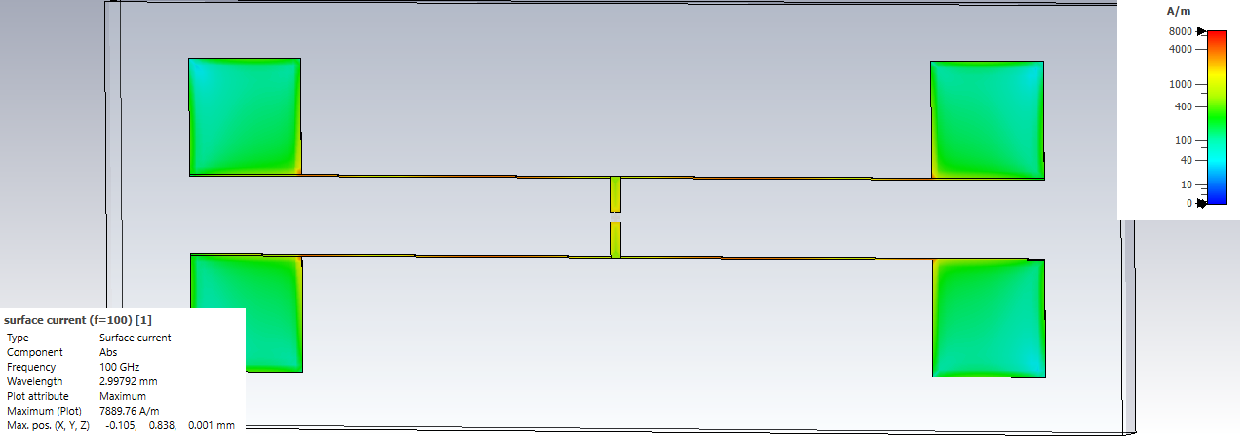
\includegraphics[width=\textwidth]{figures/contour_plots/Contour_ref_0.1THz_SC.pdf}
        \caption{}
        \label{contour_ref_100GHz}
    \end{subfigure}
    \hfill
    \begin{subfigure}[b]{1\textwidth}
        \centering
        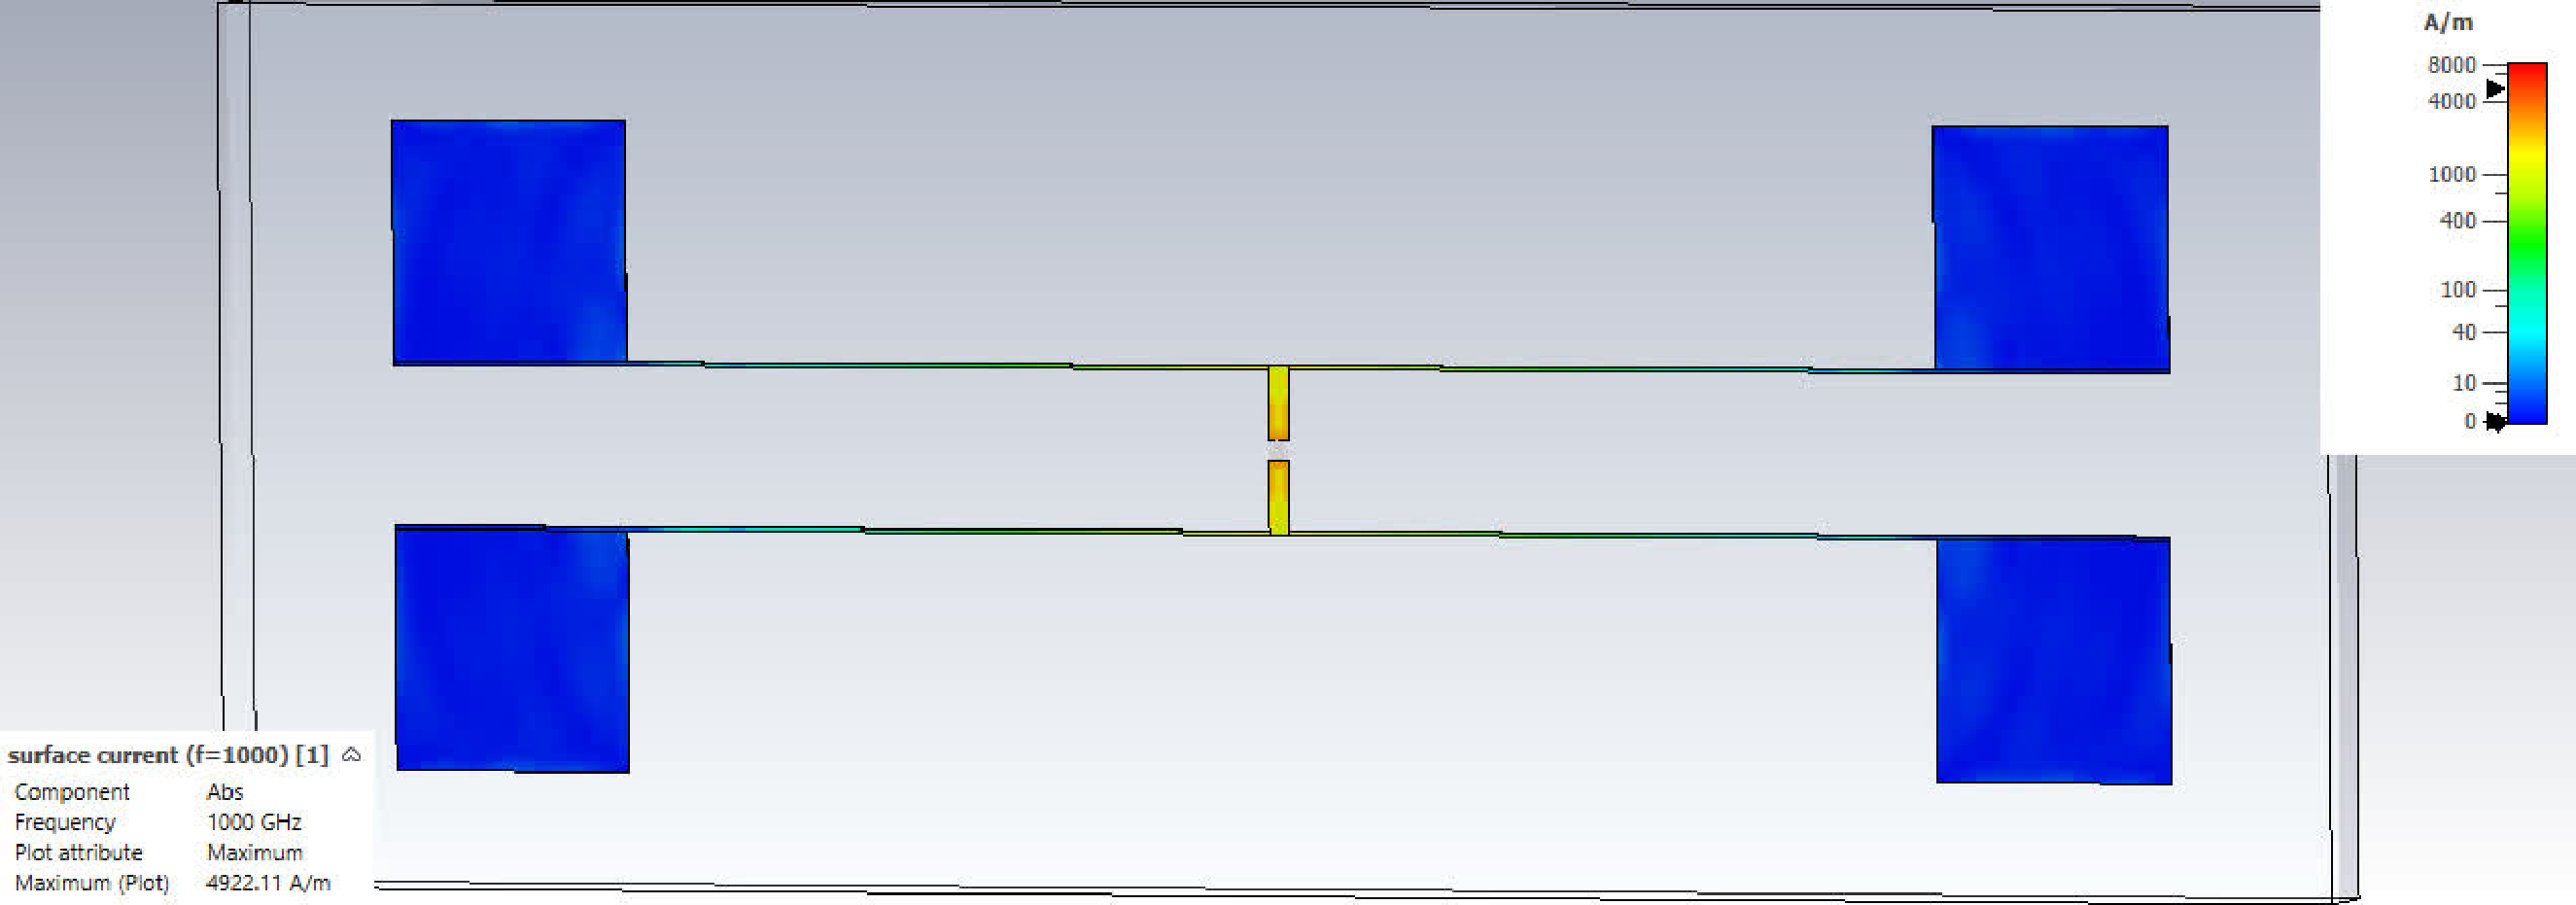
\includegraphics[width=\textwidth]{figures/contour_plots/Contour_ref_1THz_SC.pdf}
        \caption{}
        \label{contour_ref_1THz}
    \end{subfigure}
    \caption{Different PCAs and their general electrode structures are illustrated. Each antenna is designed with rectangular pads for probing. (a) Dimensions of H-Dipole electrodes. (b) Dimensions of bow-tie electrodes. (c) Dimensions of slotline antenna.}
    \label{electrodes_main}
\end{figure}






\chapter{Device Fabrication and DC Characterization}
\section{Device Fabrication Process}
\section{DC Characterization ??}

\chapter{Experimental Setup}
\section{THz TDS setup}
\section{Alignment ??}
\section{Data Analysis ??}

\chapter{Results and Discussion}

\chapter{Summary and Outlook}

\printbibliography

\end{document}
